\chapter{Can You Predict Stock Prices?}

Many arguments about investing begin with a poorly formed question:

\begin{quote}
Can stock prices be predicted accurately?
\end{quote}

The question sounds direct. It is not direct enough.

Before answering, three words must be examined: ``accurately,'' ``can,'' and ``predicted.'' What level of accuracy counts as accurate? Is the question asking whether prediction is possible in principle, or whether it is possible for ordinary investors in ordinary conditions? Who is doing the predicting, with what information, over what time span, and by what method?

This is not verbal fussiness. It is the beginning of serious thought.

A careless question invites a careless answer. If the only permitted answers are ``yes'' and ``no,'' then both may be wrong. Most important questions in money, learning, and life are not simple because their grammar is short. The right first answer is often:

\begin{quote}
It depends. Define the terms.
\end{quote}

This habit matters because investing is a field where vague thinking is expensive. The market does not forgive a person merely because his sentence sounded confident.

\section*{Simple for Whom?}

A reader once offered a useful line:

\begin{quote}
Simple things rely on intuition; complex things rely on thought.
\end{quote}

The sentence is good, but it immediately creates another question:

\begin{quote}
What counts as simple, and what counts as complex?
\end{quote}

Addition and subtraction are simple for most adults. They are not simple for a child who has just begun school. A chess position may be simple for a master and impossible for a beginner. A legal clause may be obvious to a senior lawyer and dangerous to everyone else.

The complexity of a task does not live only in the task. It also lives in the person attempting it.

Short-term stock-price prediction is a useful example. For a god with complete information, perhaps the next movement would be simple. For human beings with partial information, delayed information, emotional pressure, and competition from millions of other participants, it is not simple at all.

A person who does not understand this will treat a difficult task as if it were merely exciting. That is how gambling enters under the name of investing.

\section*{The Coin-Flip Standard}

Imagine that a stock is trading now at a known price. You are asked to predict whether its price will be higher or lower five minutes from now.

What is your expected accuracy?

For most people, under most conditions, the honest answer is close to:

\[
\frac{1}{2}
\]

That number has a harsh meaning. It means you are not predicting in any meaningful sense. You are guessing.

The minimum standard is plain:

\begin{quote}
A prediction is useful only if its accuracy is reliably higher than one half.
\end{quote}

If your accuracy is not higher than one half, a coin can replace you. If your accuracy is slightly higher than one half and the payoff structure is fair, the edge may become valuable over many repetitions. If your accuracy is high enough, say 60\%, then a long series of similar decisions can produce a strong result.

But that is exactly the problem. For the next minute, the next five minutes, the next hour, and often even the next day, most price movements are so noisy that ordinary prediction remains close to the coin-flip line.

This is uncomfortable because intuition often disagrees. We see a chart rise and feel it must continue. We see a fall and feel it must rebound. We see a pattern and feel we have discovered a law. But the feeling of pattern is not the same as a predictive edge.

The mind dislikes randomness. The market uses that dislike as raw material.

\section*{Independent Events and Bad Intuition}

One of the simplest probability lessons is also one of the hardest to accept.

If a fair coin lands heads 32 times in a row, the probability of heads on the next toss is still:

\[
\frac{1}{2}
\]

The next toss does not remember the previous tosses. Each toss is an independent event.

Many adults can recite this sentence and still fail to live by it. They secretly believe that a reversal is ``due.'' Or they believe that a streak is ``hot.'' This error is called the gambler's fallacy: the belief that previous independent outcomes should meaningfully influence the next independent outcome.

In markets, the same error wears better clothes. People say a stock must rise because it has fallen for many days. Others say it must keep rising because it has already risen so strongly. Sometimes either claim happens to be correct, but a lucky correct answer does not prove a valid method.

The difference between the gambler and the investor begins here. The gambler is ruled by patterns he has not tested. The investor asks what kind of event he is facing, what probability can reasonably be estimated, what payoff structure exists, and whether he has any edge at all.

\section*{The House Edge in Financial Costume}

Some products are designed to exploit the desire for short-term prediction. Binary options are a clear example.

The structure is simple. A platform shows a price: perhaps a stock, an index, gold, a currency pair, or a futures contract. The participant predicts whether the price will be higher or lower after one minute, five minutes, ten minutes, or fifteen minutes. If he is right, he receives a fixed payout. If he is wrong, he loses the stake.

This looks like investing only because the screen contains financial prices. In substance, it is a casino game.

Suppose a participant stakes 10. If he is wrong, he loses 10. If he is right, the total return may be 18, including his original stake. The winning side feels attractive because the screen says ``80\% return.'' The full structure says something else: the house keeps an edge.

A compact expected-value model is enough:

\[
\text{Expected return}
=
p \times \text{winning payout}
-
(1-p) \times \text{loss}
\]

where \(p\) is the probability of being correct.

If the participant has no real edge, then \(p\) is close to \(1/2\). In that case the game is not neutral; the payout rules make it negative. The more often he plays, the more reliably the structure collects from him.

This is why a person can have several wins and still be walking toward ruin. A few lucky outcomes do not change the system. When the house edge is large, the participant must achieve a prediction accuracy far above ordinary guessing just to survive. In practice, the product demands what the participant does not possess: reliable short-term prediction.

The casino is honest enough to look like a casino. A financial casino is more dangerous because it lets the participant call himself an investor.

\section*{Overall Results Matter}

Probability requires the discipline to look at the whole set, not only at the visible story.

There may be individuals who win in a gambling-like product for a while. Some may even leave with a profit. That does not make the product favorable. The question is:

\begin{quote}
What happens to the total group over enough repetitions?
\end{quote}

If the total group loses in a pattern that matches the house edge, then the occasional winner is not evidence against the rule. He is part of the distribution. He is the person randomness temporarily placed above the average.

This is why statistical thinking is one of the most basic money-thinking tools. Not one useful tool among many, but one of the foundations. Without it, a person mistakes anecdotes for laws, streaks for skill, confidence for evidence, and survivorship for proof.

A person who wants to invest but refuses to learn probability is like someone entering the sea without equipment because the surface looks calm.

\section*{Random Walk and Its Proper Range}

In finance there is a famous idea called the random walk hypothesis. In its rough form, it says that stock prices move in a pattern that cannot be predicted reliably.

The idea has a long history. It appeared in early form in nineteenth-century work, was developed mathematically in the twentieth century, and became widely known through Burton Malkiel's \emph{A Random Walk Down Wall Street}. It remains controversial, partly because people use the same phrase to talk about different time horizons.

A more useful version is this:

\begin{enumerate}
\item Short-term price prediction is extremely difficult, often practically impossible.
\item Long-term price judgment is possible.
\item The longer the time horizon, the more important fundamentals become.
\end{enumerate}

This version removes much of the unnecessary argument.

Predicting whether a strong company will trade higher five minutes from now is nearly meaningless. Predicting whether a strong company, in a growing economy, with durable advantages, may be worth much more in five or ten years is a different task. The second task is still uncertain, but it is not the same kind of uncertainty.

Short time spans are dominated by noise, liquidity, emotion, positioning, news, rumor, and random order flow. Long time spans give business reality more room to appear: revenue, profit, reinvestment, competition, management, network effects, technology shifts, regulation, and economic growth.

The investor must not confuse these two worlds.

\begin{center}
\begin{adjustbox}{max width=\linewidth}
\begin{tikzpicture}[font=\scriptsize, >=stealth, node distance=1cm]
\node[draw, rounded corners=2pt, align=center, minimum width=2.4cm] (short) {Minutes\\days};
\node[draw, rounded corners=2pt, align=center, right=of short, minimum width=2.4cm] (medium) {Months\\years};
\node[draw, rounded corners=2pt, align=center, right=of medium, minimum width=2.4cm] (long) {Many\\years};
\node[align=center, below=.55cm of short] (s1) {noise\\dominates};
\node[align=center, below=.55cm of medium] (s2) {mixed\\signals};
\node[align=center, below=.55cm of long] (s3) {fundamentals\\matter more};
\draw[->] (short) -- (medium);
\draw[->] (medium) -- (long);
\end{tikzpicture}
\end{adjustbox}
\end{center}

The practical rule is:

\begin{quote}
Do not hold excessive expectations for the short term, and do not hold insufficient expectations for the long term.
\end{quote}

Most people do the reverse. They want the next week to change their lives, but they cannot imagine what ten disciplined years may produce. They overpay for excitement and underpay for compounding.

\section*{Why Long-Term Prediction Can Be Easier}

At first, it sounds strange to say that distant prediction can be easier than near prediction. Yet in investing, this can be true.

Ask whether a particular stock will be higher five minutes from now. The answer is mostly noise.

Ask whether the value of a strong business can grow over many years if it operates in a growing market, serves real demand, allocates capital well, and keeps its competitive position. The question is still difficult, but it has substance. You can study the business. You can examine the industry. You can compare competitors. You can read reports. You can watch user behavior. You can revise your thesis as facts change.

The stock price ultimately follows business value imperfectly, with delays, exaggerations, and surprises. But over a long enough horizon, value has more influence than momentary emotion.

This is why some long-term judgments are easier than short-term guesses. They are not easier because the future is certain. They are easier because the relevant causes are more knowable.

The image to keep in mind is not a straight line. It is a noisy path around a direction.

\begin{center}
\begin{adjustbox}{max width=\linewidth}
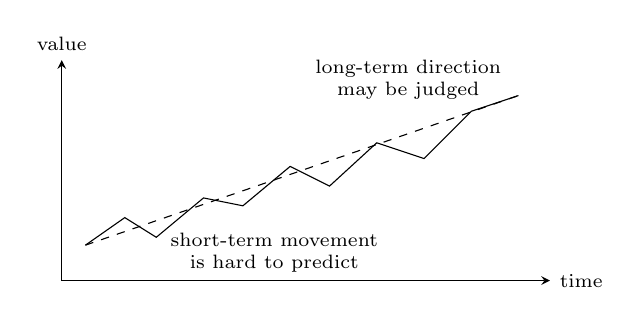
\begin{tikzpicture}[font=\scriptsize, x=1cm, y=1cm, >=stealth]
\draw[->] (0,0) -- (6.2,0) node[right] {time};
\draw[->] (0,0) -- (0,2.8) node[above] {value};
\draw[thin] (0.3,.45) -- (.8,.8) -- (1.2,.55) -- (1.8,1.05) -- (2.3,.95) -- (2.9,1.45) -- (3.4,1.2) -- (4.0,1.75) -- (4.6,1.55) -- (5.2,2.15) -- (5.8,2.35);
\draw[dashed] (0.3,.45) -- (5.8,2.35);
\node[align=center] at (2.7,.35) {short-term movement\\is hard to predict};
\node[align=center] at (4.4,2.55) {long-term direction\\may be judged};
\end{tikzpicture}
\end{adjustbox}
\end{center}

The dashed line is not guaranteed. It is a thesis. The jagged line is the experience of ownership.

\section*{Knowledge Must Change Behavior}

It is not enough to understand these ideas intellectually.

Many people know a sentence but do not believe it deeply enough to act differently. They say effort matters but do not work. They say health matters but do not change habits. They say long-term investing matters but check prices every hour. They say short-term prediction is impossible, then spend attention trying to do it.

Knowledge that does not change behavior is not yet real knowledge for that person.

This is where metacognition returns. The point is not merely to learn the phrase ``random walk.'' The point is to observe yourself when the market moves. Do you feel pulled into prediction? Do you want to check again? Do you become proud after a correct guess? Do you become ashamed after a wrong one? Do you confuse a lucky outcome with a strengthened method?

If a concept is true for you, it changes the design of your life.

That is why the previous chapter's practice of updating investment records monthly is not a small technical suggestion. It is a behavioral design. It trains the mind away from short-term noise. It sentences capital and attention to a longer term. It teaches the investor to stop feeding the part of the mind that wants stimulation.

The discipline may take a year to become natural. A year is cheap. Losing capital and attention for decades is expensive.

\section*{The Difference Between Investor and Gambler}

An exchange and a casino share one surface feature: people place money under uncertainty. Trading volume can even be compared to total betting volume, and transaction costs resemble the house's collection.

But there is still a decisive difference between a gambler and an investor.

The gambler seeks action without a durable edge. He wants excitement, rescue, proof, or escape. He is attracted to short intervals because short intervals offer frequent emotional feedback.

The investor seeks a favorable long-term relation between price, value, probability, and time. He does not need every short-term movement to explain itself. He does not demand stimulation from the market. He is willing to be bored if boredom protects judgment.

A pocket model is enough:

\begin{center}
\begin{adjustbox}{max width=\linewidth}
\begin{tabular}{p{0.28\linewidth}p{0.29\linewidth}p{0.29\linewidth}}
\hline
Question & Gambler & Investor \\
\hline
Time horizon & Minutes or days & Years or longer \\
Core desire & Excitement or quick rescue & Compounding and ownership \\
Basis of action & Feeling, streak, rumor & Thesis, evidence, sizing \\
View of loss & Bad luck or betrayal & Information and risk cost \\
Use of attention & Constant checking & Scheduled review \\
\hline
\end{tabular}
\end{adjustbox}
\end{center}

The same person can be an investor in one decision and a gambler in another. The label is not permanent. It is earned by behavior.

\section*{Do the Necessary Homework}

Probability and statistics are not decorative subjects. They are part of the basic equipment of adulthood, especially for anyone who wants to handle capital.

Many people need to repair this foundation. They need to understand hypotheses, theories, principles, independent events, expected value, variance, outliers, sample size, base rates, survivorship bias, and logical fallacies. They also need to stop treating ``controversial'' as a synonym for ``false.'' Many true or useful ideas remain controversial because they are hard to understand, emotionally inconvenient, or applied carelessly.

No single recommended book can replace the habit of learning. A university-level probability and statistics textbook is already enough for a beginning. More important, choosing what to study is itself a skill. If every learning decision must be outsourced, the ability to choose will weaken.

Keep an open mind across fields. Finance borrows from mathematics, psychology, accounting, law, history, technology, and human nature. The larger your mental toolbox, the less helpless you become when reality changes shape.

\section*{Knowledge Is Money, Time Is Power}

The old sentence says:

\begin{quote}
Knowledge is power; time is money.
\end{quote}

For investors, it is often more accurate to reverse it:

\begin{quote}
Knowledge is money; time is power.
\end{quote}

Knowledge is money because concepts determine decisions, and decisions determine capital outcomes. A person who understands expected value avoids games designed to drain him. A person who understands independent events avoids the gambler's fallacy. A person who understands long horizons stops wasting attention on meaningless fluctuations.

Time is power because compounding needs duration, and duration changes the meaning of ordinary growth. The longer the sentence you give your capital, the more room knowledge has to work. This is why assigning money to a long term changes the investor himself. It reduces the demand for immediate proof. It weakens the addiction to short-term prediction. It makes patience practical rather than ornamental.

The chapter's rule can be stated simply:

\begin{quote}
Avoid short-term prediction unless you can prove a real edge; build long-term judgment where fundamentals, probability, and time can work together.
\end{quote}

This rule is not exciting. That is part of its value. Wealth freedom is not built by being excited more often. It is built by seeing more clearly, deciding more carefully, and letting time apply force to correct behavior.
